\documentclass[12pt]{article}
\usepackage{graphicx}
\usepackage{latexsym}              % symbols
\usepackage{amsmath}               % great math stuff
\usepackage{amssymb}               % great math symbols
\usepackage{amsfonts}              % for blackboard bold, etc
\usepackage{amsthm}                % for theorems
\usepackage{graphicx}              % for insert graph
\usepackage{listings}              % for code block

\lstset{frame=tb,
  language=Java,
  aboveskip=3mm,
  belowskip=3mm,
  showstringspaces=false,
  columns=flexible,
  basicstyle={\small\ttfamily},
  numbers=none,
  numberstyle=\tiny,
  breaklines=true,
  breakatwhitespace=true,
  tabsize=3
}


\newcommand{\N}{\mathbb{N}}
\newcommand{\Z}{\mathbb{Z}}
\newcommand{\R}{\mathbb{R}}
\newcommand{\C}{\mathbb{C}}
\newcommand{\F}{\mathbb{F}}

\renewcommand{\vert}{\,|\,}
\newcommand{\mb}{\textbf}
\newcommand{\norm}[2]{\|{#1}\|_{#2}}
\newcommand{\normm}[1]{\|#1\|}
\newcommand{\bmat}[1]{\begin{bmatrix} #1 \end{bmatrix}}
\newcommand{\pmat}[1]{\begin{pmatrix} #1 \end{pmatrix}}
\newcommand{\eqtext}[1]{\hspace{3mm} \text{#1} \hspace{3mm}}
\newcommand{\set}[1]{\{#1\}}
\newcommand{\inn}[2]{\langle #1, #2 \rangle}
\newcommand{\ra}{\rightarrow}
\newcommand{\Ra}{\Rightarrow}
\newcommand{\tx}[1]{\text{{#1}}}
\newcommand{\abs}[1]{|#1|}
\newcommand{\bigO}{\mathcal{O}}
% \newcommand{\det}{\text{det}}
\DeclareMathOperator{\E}{\mathbb{E}}

\DeclareMathOperator{\E}{\mathbb{E}}
\DeclareMathOperator{\J}{\mathcal J^\beta_\tx{reg}}

\begin{document}
  CSC311 A2
  \hfill
  Guanglei Zhu
  \smallskip
  \hrule
  \bigskip
  \begin{enumerate}
    \item \begin{enumerate}
    \item $$\E[\mathcal{L}(y=\tx{keep}, t)] = 0.1 \cdot 1 + 0.9 \cdot 0 = 0.1$$
    $$\E[\mathcal{L}(y=\tx{keep}, t)] = 0.1 \cdot 0 + 0.9 \cdot 100 = 90$$
    \item \begin{align*}
    &\E[\mathcal{L}(y=\tx{keep}, t) \, | \, x]   \\
    =& 1 \cdot \tx{Pr}(t = \tx{spam}\, |\, x) + 0 \cdot (1 - \tx{Pr}(t = \tx{spam}\, |\, x)) \\
    =& \tx{Pr}(t = \tx{spam}\, |\, x)
    \end{align*}
    \begin{align*}
    &\E[\mathcal{L}(y=\tx{remove}, t) \, | \, x]   \\
    =& 0 \cdot \tx{Pr}(t = \tx{spam}\, |\, x) + 100 \cdot (1 - \tx{Pr}(t = \tx{spam}\, |\, x)) \\
    =& 100 \cdot (1 - \tx{Pr}(t = \tx{spam}\, |\, x))
    \end{align*}
    If $\tx{Pr}(t = \tx{spam}\, |\, x) \leq 100 \cdot (1 - \tx{Pr}(t = \tx{spam}\, |\, x))$, then choose $y_* = \tx{keep}$, else $y_* = \tx{remove}$.
    \item
    By Bayes rule, we know that $$\tx{Pr}(t = \tx{spam}\, |\, (x_1, x_2)) = \frac{\tx{Pr}(t = \tx{spam}) \cdot \tx{Pr}(x_1, x_2 \, | \, t = \tx{spam})}{\tx{Pr}(x_1, x_2)}$$
    $$\tx{Pr}(t = \tx{spam}\, |\, (0, 0)) = \frac{0.4 \cdot 0.1}{0.1 \cdot 0.4 + 0.9 \cdot 0.998} = 0.043$$
    $$\tx{Pr}(t = \tx{spam}\, |\, (0, 1)) = \frac{0.3 \cdot 0.1}{0.1 \cdot 0.3 + 0.9 \cdot 0.001} = 0.971$$
    $$\tx{Pr}(t = \tx{spam}\, |\, (1, 0)) = \frac{0.2 \cdot 0.1}{0.1 \cdot 0.2 + 0.9 \cdot 0.001} = 0.957$$
    $$\tx{Pr}(t = \tx{spam}\, |\, (1, 1)) = \frac{0.1 \cdot 0.1}{0.1 \cdot 0.1 + 0.9 \cdot 0} = 1$$
    According to part (b), $y_* =
    \begin{cases} \tx{ remove} \qquad (x_1, x_2) = (1, 1)\\ \tx{ keep} \qquad \quad \tx{ else}
    \end{cases}$
    \item \begin{align*}
      \E[\mathcal{L}(y_*), t] =& \, \mathcal{L}(\tx{keep}, \tx{spam}) \cdot
      \tx{Pr}(t = \tx{spam}\, |\, (0, 0)) \cdot \tx{Pr}(\textbf x = (0, 0)) \\
      &+ \mathcal{L}(\tx{keep}, \tx{spam}) \cdot
      \tx{Pr}(t = \tx{spam}\, |\, (0, 1)) \cdot \tx{Pr}(\textbf x = (0, 1)) \\
      &+ \mathcal{L}(\tx{keep}, \tx{spam}) \cdot
      \tx{Pr}(t = \tx{spam}\, |\, (1, 0)) \cdot \tx{Pr}(\textbf x = (1, 0)) \\
      &+ \mathcal{L}(\tx{remove}, \tx{non-spam}) \cdot
      \tx{Pr}(t = \tx{non-spam}\, |\, (1, 1)) \cdot \tx{Pr}(\textbf x = (1, 1)) \\
      =& \, 1 \cdot 0.043 \cdot 0.9382 + 1 \cdot 0.971 \cdot 0.0309 + 1 \cdot 0.957 \cdot 0.0209
      + 0 \\
      =& \, 0.09
  \end{align*}
  \end{enumerate}
  \item \begin{enumerate}
    \item Suppose the dataset is linearly separable, since $x = -1$ and $x = 3$ both have label 1, any point between them should also have label 1. In particular, $x = 1$ should also have label $t = 1$ which leads to contradiction. Therefore, the data is not linearly separable.
    \item From the feature map, we get
    $$\psi(-1) = \pmat{-1 \\ 1}, \psi(1) = \pmat{1 \\ 1}, \psi(3) = \pmat{3 \\ 9}$$
    the constraint on $w_1, w_2$ is
    \begin{center}
      $\begin{cases}
        -w_1 + w_2 \geq 0 \\
        w_1 + w_2 < 0 \\
        3w_1 + 9w_2 \geq 0
      \end{cases}$
    \end{center}  $\Rightarrow (w_1, w_2) = (-2, 1)$ correctly classify all the examples.
    \end{enumerate}
    \item[3.1.] \begin{enumerate}
    \item here is the plot on validation set:
    \begin{center}
      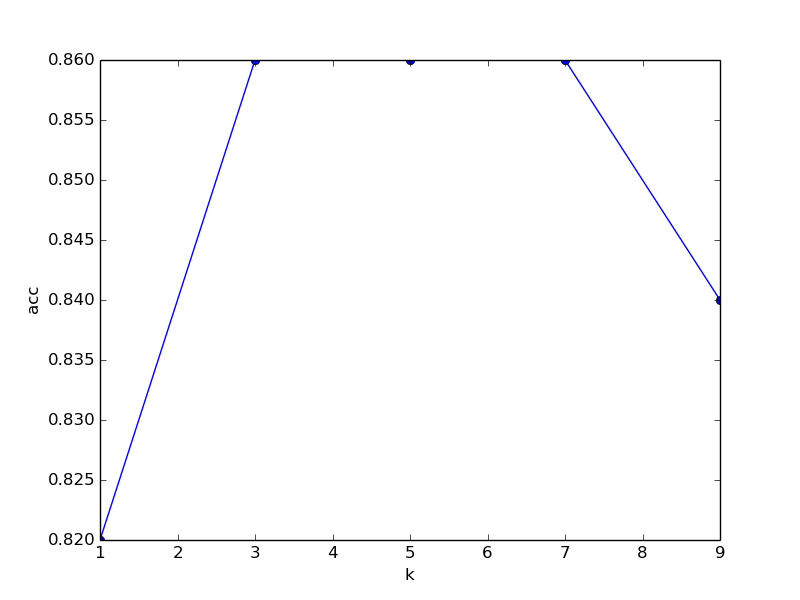
\includegraphics[scale=0.5]{q3/q3_1a.png}
    \end{center}
    \item The performance of knn on this data set is reasonably well, for many choice of $k$, the classification rate is over 85\%. \\ My choice is $k^* = 5$, here is the test classification rate:
    \begin{center}
      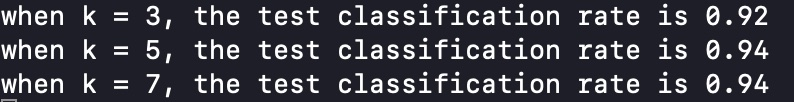
\includegraphics[scale=0.3]{q3_1b.jpg}
    \end{center}
    It's easy to see that the test performance of these values of $k$
    is better than the validation performance.
    \end{enumerate}
    \item[3.2.] \begin{enumerate}
        \item[(b)] For data set \texttt{mnist\_train}:
        \begin{center}
          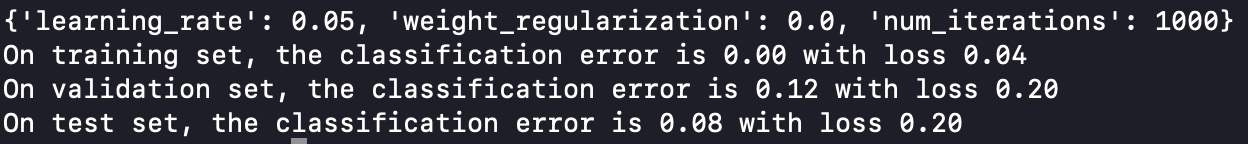
\includegraphics[scale=0.3]{q3_2b_1.jpg}
        \end{center}
        For data set \texttt{mnist\_train\_small}:
        \begin{center}
          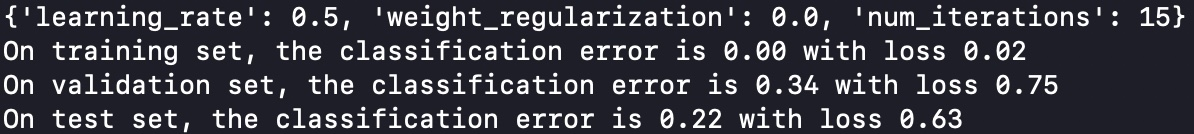
\includegraphics[scale=0.3]{q3_2b_2.jpg}
        \end{center}
        \item[(c)] For data set \texttt{mnist\_train}:
        \begin{center}
          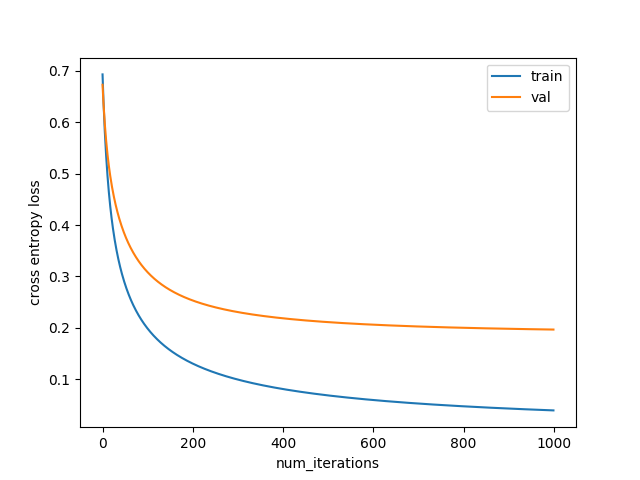
\includegraphics[scale=0.7]{q3/q3_2c_1.png}
        \end{center}
        \texttt{learning\_rate = 0.05}, \texttt{iterations = 1000} \\
        The higher the learning rate, the faster the graph converges. However, if the learning rate is too high, it might cause higher cross entropy loss. Low learning rate will take more iterations to converges.
        \newpage
        For data set \texttt{mnist\_train\_small}:
        \begin{center}
          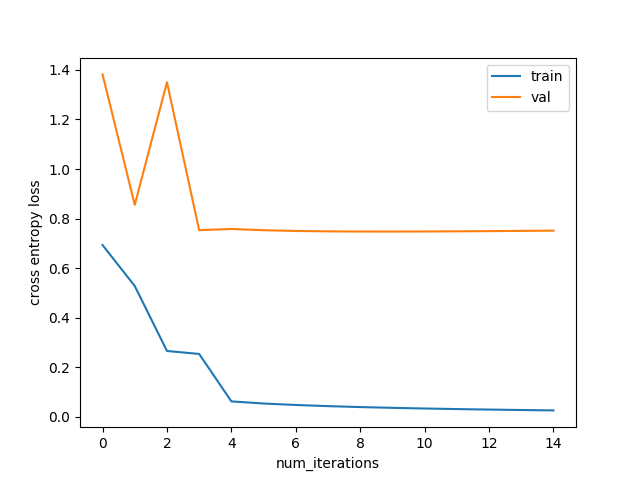
\includegraphics[scale=0.7]{q3/q3_2c_2.png}
        \end{center}
        \texttt{learning\_rate = 0.5}, \texttt{iterations = 15} \\
        Since it's a small data set, when the iterations is too large (over 20), the validation loss is increasing while the training loss is decreasing which indicates overfitting. If the learning rate is too high (over 2), it will lead numerical instability.
    \end{enumerate}
    \item[4.] \begin{enumerate}
      \item Let $f = \frac 1 2 \displaystyle\sum_{i=1}^N a^{(i)}(y^{(i)}-\mb w^T \mb x^{(i)})^2 + \frac \lambda 2 \sum_{i=1}^N w_i^2$, differentiate wrst. $w_j$
      \begin{align*}
        \frac{\partial f}{\partial w_j} &= \sum_{i=1}^N a^{(i)}(y^{(i)}-\mb w^T \mb x^{(i)})(-x_j^{(i)}) + \lambda w_j \\
        &= \sum_{i=1}^N a^{(i)}x_j^{(i)}(\sum_{k=1}^D w_k x_k^{(i)} - y^{(i)}) + \lambda w_j \\
        &= \sum_{i=1}^N a^{(i)}x_j^{(i)}\sum_{k=1}^D w_k x_k^{(i)} - \sum_{i=1}^N a^{(i)}x_j^{(i)} y^{(i)} + \lambda w_j \\
        &= \sum_{k=1}^D w_k \sum_{i=1}^N a^{(i)}x_j^{(i)} x_k^{(i)} - \sum_{i=1}^N a^{(i)}x_j^{(i)} y^{(i)} + \lambda w_j  \\
        &= \sum_{k=1}^D w_k (\lambda I(j = k) + \sum_{i=1}^N a^{(i)}x_j^{(i)} x_k^{(i)}) - \sum_{i=1}^N a^{(i)}x_j^{(i)} y^{(i)}
      \end{align*}
      Let $A_{jk} = \lambda I(j = k) + \sum_{i=1}^N a^{(i)}x_j^{(i)} x_k^{(i)}$ and
      $c_j = \sum_{i=1}^N a^{(i)}x_j^{(i)} y^{(i)}$.
      Similar to A1 Q3, by observation,
      $$\frac{\partial f}{\partial w_j} = \mb B \mb w - \mb c \overset{set}{=} 0$$
      where $\mb B = \mb X^T \mb A \mb X + \lambda \mb I$ and $\mb c = \mb X^T \mb A \mb y$. Therefore,
      $$\mb w^* = (\mb X^T \mb A \mb X + \lambda \mb I)^{-1} \mb X^T \mb A \mb y$$
      \item[(c)] Here is the validation losses as a function of $\tau$
      \begin{center}
        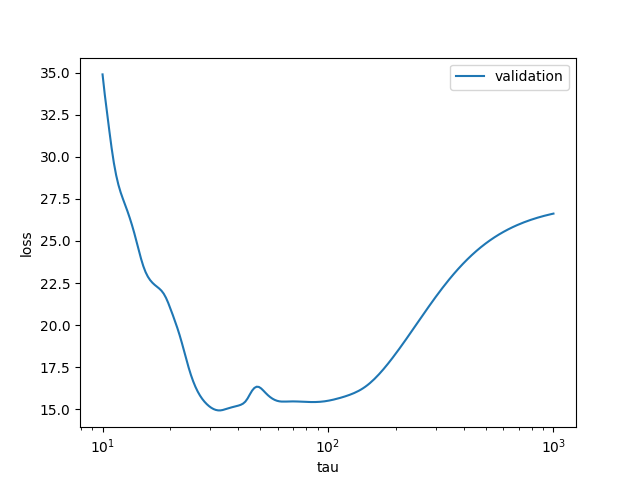
\includegraphics[scale=0.7]{q4.png}
      \end{center}
      \item[(d)] The validation loss will be high as $\tau \rightarrow \infty$ and $\tau \rightarrow 0.$ When $\tau \rightarrow \infty$, the validation loss converges to a constant number.
      As $\tau \rightarrow \infty , a^{(i)} \rightarrow 1/N$ and the model becomes a linear regression model which is invariant of $\tau$.
      As $\tau \rightarrow 0$, the training loss is almost 0 which indicates overfitting and causes high loss.
      \begin{center}
        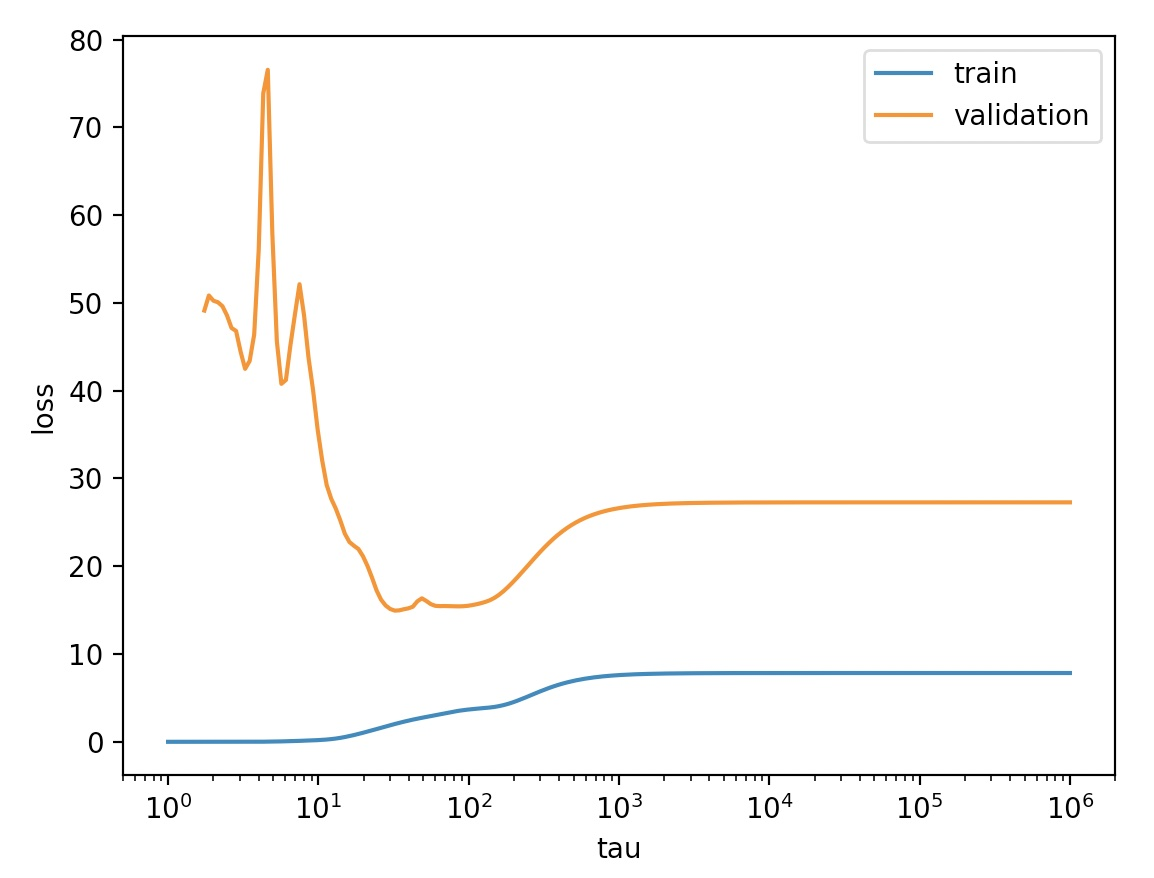
\includegraphics[scale=0.3]{q4d.jpg}
      \end{center}
      The plot, as $\tau$ ranges from $10^0$ to $10^6$, also supports this argument.
  \end{enumerate}
  \end{enumerate}
\end{document}
